% Shared standalone design for the editable figure reconstructions.
\documentclass[tikz,border=5pt,10pt]{standalone}
\usepackage[T1]{fontenc}
\usepackage[utf8]{inputenc}
\usepackage{newpxtext,newpxmath}
\usepackage[scaled=.94]{sourcesanspro}
\usepackage{pgfplots}
\pgfplotsset{compat=1.18}
\usetikzlibrary{arrows.meta,calc,positioning,decorations.pathreplacing,
  decorations.markings,patterns,matrix,shapes.geometric,fit,backgrounds,
  intersections,angles,quotes}
\definecolor{ink}{HTML}{203746}
\definecolor{accent}{HTML}{146C78}
\definecolor{muted}{HTML}{667780}
\definecolor{signalred}{HTML}{B94B44}
\color{ink}
\tikzset{>=Latex,line width=.8pt,
  every node/.style={font=\small},
  axis/.style={->,draw=muted,line width=.5pt},
  guide/.style={draw=muted,dashed,line width=.45pt},
  curve/.style={draw=accent,line width=1pt},
  marker/.style={circle,fill=accent,inner sep=1.5pt},
  labelbox/.style={fill=white,inner sep=2pt}}

\begin{document}
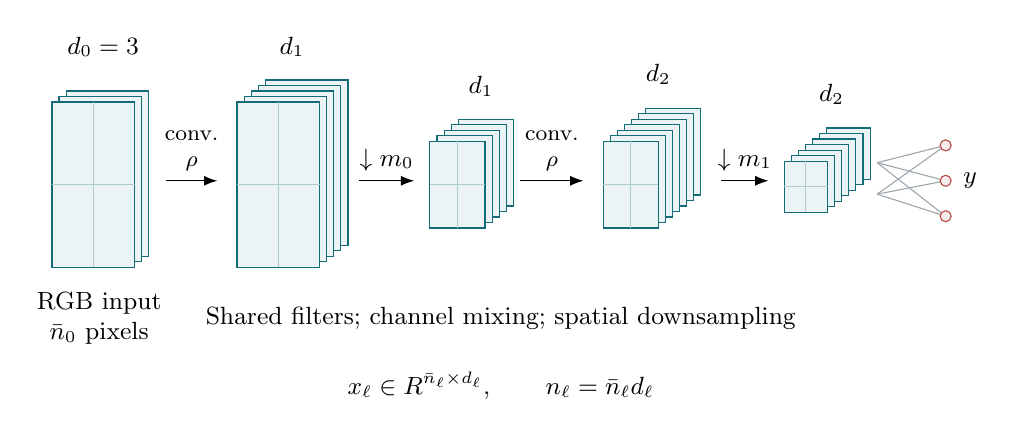
\begin{tikzpicture}[x=1cm,y=1cm]
\newcommand{\featurestack}[5]{\begin{scope}[shift={(#1,#2)}]
\foreach \k in {#5,...,0}{\path[draw=accent,fill=accent!8]({.09*\k},{.07*\k})rectangle({#3+.09*\k},{#4+.07*\k});}
\draw[accent!35,line width=.3pt](0,{#4/2})--(#3,{#4/2});\draw[accent!35,line width=.3pt]({#3/2},0)--({#3/2},#4);
\end{scope}}
\featurestack{0}{0}{1.05}{2.1}{2}
\featurestack{2.35}{0}{1.05}{2.1}{4}
\featurestack{4.8}{.5}{.7}{1.1}{4}
\featurestack{7.0}{.5}{.7}{1.1}{6}
\featurestack{9.3}{.7}{.55}{.65}{6}
\node at(.65,2.8){$d_0=3$};\node at(3.05,2.8){$d_1$};\node at(5.45,2.3){$d_1$};\node at(7.7,2.45){$d_2$};\node at(9.9,2.2){$d_2$};
\draw[->](1.45,1.1)--(2.1,1.1)node[midway,above,align=center,font=\footnotesize]{conv.\\$\rho$};
\draw[->](3.9,1.1)--(4.6,1.1)node[midway,above]{$\downarrow m_0$};
\draw[->](5.95,1.1)--(6.75,1.1)node[midway,above,align=center,font=\footnotesize]{conv.\\$\rho$};
\draw[->](8.5,1.1)--(9.1,1.1)node[midway,above]{$\downarrow m_1$};
\foreach \y in {.65,1.1,1.55}{\draw[muted!65](10.48,.93)--(11.35,\y);\draw[muted!65](10.48,1.33)--(11.35,\y);\filldraw[draw=signalred,fill=signalred!10](11.35,\y)circle(.07);}
\node[right]at(11.45,1.1){$y$};
\node[align=center]at(.6,-.65){RGB input\\$\bar n_0$ pixels};
\node[align=center]at(5.7,-.65){Shared filters; channel mixing; spatial downsampling};
\node at(5.7,-1.5){$x_\ell\in\mathbb R^{\bar n_\ell\times d_\ell},\qquad n_\ell=\bar n_\ell d_\ell$};
\end{tikzpicture}
\end{document}
